\chapter{Metodologia}
\label{cap:metodologia}

Este capítulo descreve o caminho adotado para conduzir o trabalho e para avaliar se a solução proposta atende ao problema identificado. Seguindo uma organização top-down, a metodologia apresenta primeiro a natureza da pesquisa, depois os procedimentos de desenvolvimento e, por fim, a estratégia de avaliação do protótipo.

\section{Caracterização da Pesquisa}

O trabalho caracteriza-se como uma pesquisa aplicada de natureza tecnológica, pois tem como objetivo produzir uma solução computacional para apoiar um processo acadêmico real: a organização e a pré-validação do barema de atividades complementares do Colegiado de Ciência da Computação. A pesquisa possui abordagem qualitativa, uma vez que parte da análise do fluxo utilizado pelos discentes, das regras institucionais e das dificuldades observadas na preparação dos documentos.

O foco do estudo não é propor um novo método teórico de avaliação acadêmica, mas transformar regras já existentes em uma ferramenta funcional. Assim, o mérito do trabalho está na construção, organização e validação de um protótipo capaz de reduzir erros recorrentes no preenchimento, anexação e conferência inicial dos certificados.

\section{Procedimentos Metodológicos}

O desenvolvimento foi conduzido por prototipagem evolutiva, em que versões sucessivas do sistema foram refinadas a partir das necessidades identificadas durante o levantamento e a implementação \cite{soares2007}. Essa estratégia foi adotada porque o problema envolve interação com usuário, regras de negócio específicas e tratamento de documentos em formato PDF, aspectos que exigem ajustes progressivos ao longo do desenvolvimento.

A abordagem evolutiva permitiu organizar o trabalho em ciclos de compreensão do problema, modelagem da solução, implementação, testes e refinamento. Em vez de tratar o sistema como um produto definido integralmente desde o início, cada ciclo incorporou novas regras, ajustes de usabilidade e melhorias técnicas observadas durante a construção do protótipo. A Figura~\ref{fig:fluxo-desenvolvimento} sintetiza esse fluxo de desenvolvimento adotado no trabalho.

\begin{figure}[H]
    \centering
    \caption{Fluxo do ciclo de desenvolvimento adotado}
    \label{fig:fluxo-desenvolvimento}
    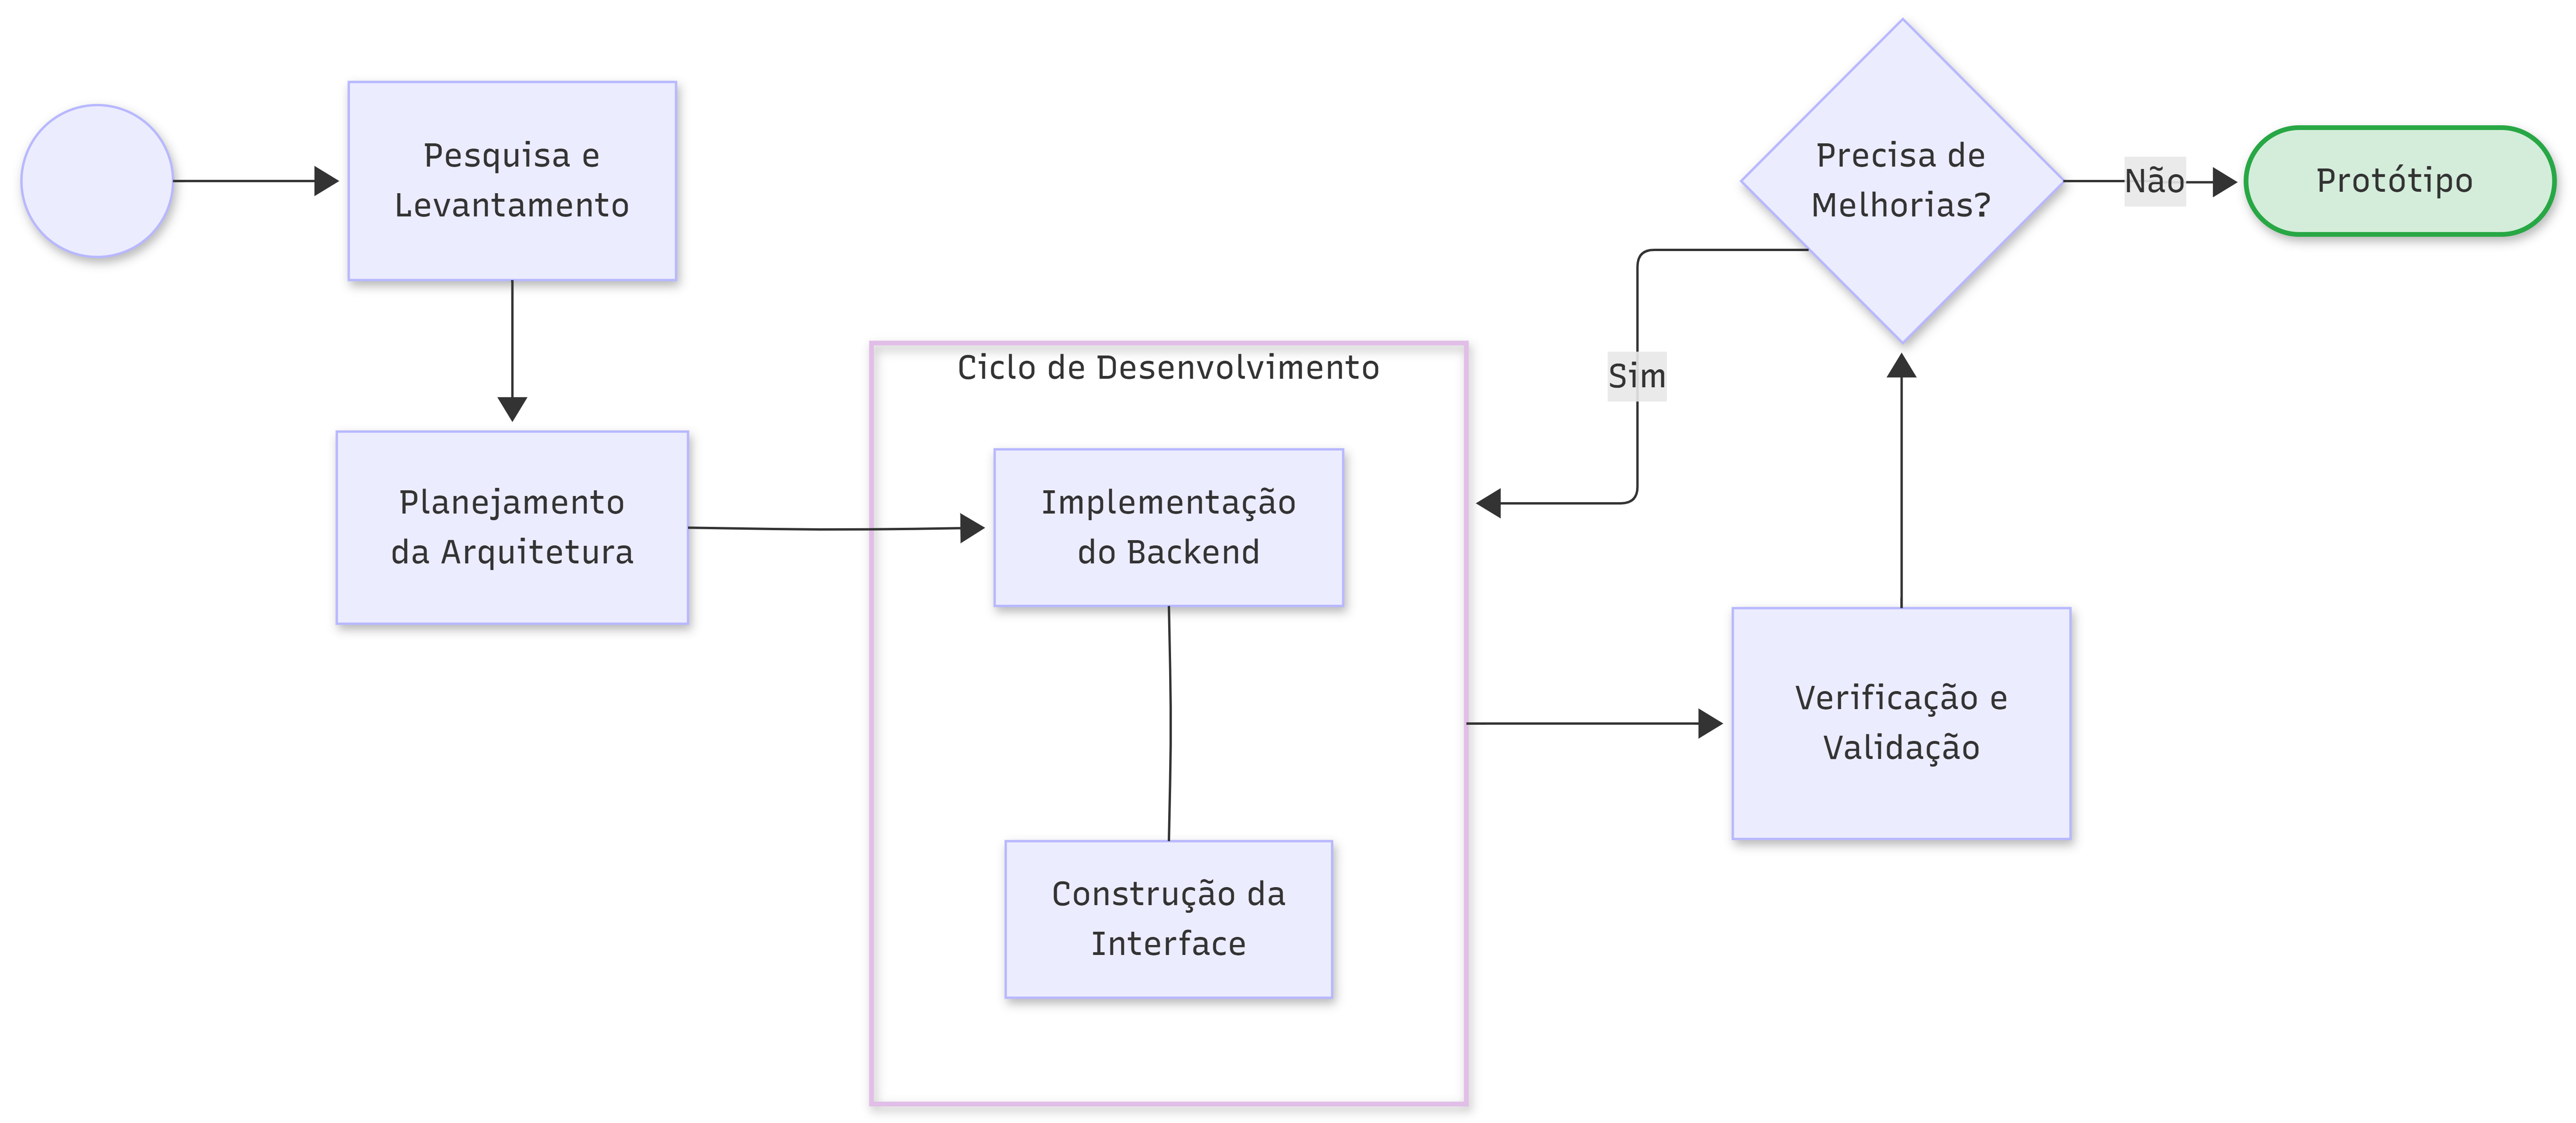
\includegraphics[width=0.95\textwidth]{figuras/fluxo_desenvolvimento.png}
    \legend{Fonte: elaboração própria.}
\end{figure}

Inicialmente, foi realizado o levantamento das regras do barema e das informações necessárias para compor a solicitação do discente. Em seguida, definiu-se a estrutura geral do sistema, incluindo a separação entre interface, rotas da aplicação, serviços de processamento, regras de validação e geração do documento final. Na etapa de implementação, foram desenvolvidos os mecanismos de preenchimento do formulário, anexação de certificados, extração de informações dos arquivos, pré-validação e montagem do PDF consolidado.

Durante o desenvolvimento, as funcionalidades foram testadas de forma incremental. A cada novo recurso, foram verificados os efeitos sobre o fluxo completo de uso, evitando que decisões de implementação ficassem desconectadas do objetivo central do sistema.

\section{Estratégia de Avaliação}

A avaliação do protótipo foi planejada com base em testes funcionais e em critérios de conformidade com as regras do barema. Foram considerados cenários como anexação de múltiplos certificados, identificação de carga horária, comparação entre horas solicitadas e horas comprovadas, detecção de certificados duplicados, geração do documento final e funcionamento da pré-validação.

Também foi prevista a verificação do comportamento do sistema diante de limitações do processamento automático, como certificados sem texto extraível ou indisponibilidade de serviços externos de inteligência artificial. Nesses casos, a avaliação observa se o sistema mantém um comportamento seguro, recorrendo à validação básica quando necessário.

Dessa forma, a avaliação busca responder se o protótipo reduz erros antes da submissão oficial, mantém aderência às regras do COLCIC e produz um documento final organizado para análise posterior.
